\chapter{Recap}
\pagebreak
% Describe process states with state diagram.

% Explain the CPU switch from process to process with an appropriate diagram.

% Explain single and multithreaded processes showing different types of multithreading models.

% Explain different types of schedulers using queuing diagram of process scheduling.


\begin{multicols}{2}
\subsection*{Interrupt}

An interrupt is a signal sent to the processor that interrupts the current process, generated by hardware devices (e.g., mouse, keyboard) or software programs. An operating system is interrupt driven.

\textbf{Common Functions of Interrupts}
\begin{itemize}[topsep=-0.5em, parsep=0.5em]
   \item Interrupt \rgbR{transfers control} to the interrupt service routine generally, through the \textbf{interrupt vector}, which contains the addresses of all the service routines.
   
   \item Interrupt \rgbR{architecture must save} the address of the interrupted instruction.
   
   \item \rgbR{Incoming interrupts} are disabled while another interrupt is being processed to prevent a lost interrupt.
   
   \item A \rgbR{trap} is a software-generated interrupt caused either by an error or a user request.
\end{itemize}

\textbf{Interrupt Handling}
\begin{itemize}[topsep=-0.5em, parsep=0.5em]
   \item	\rgbR{OS preserves} CPU state by storing registers and program counter.
   \item	Determines \rgbR{interrupt type}: polling or vectored interrupt system.
   \item	Separate \rgbR{code segments define} actions for each interrupt type.
\end{itemize}

\subsection*{Memory}
\begin{figure}[H]
   \centering
   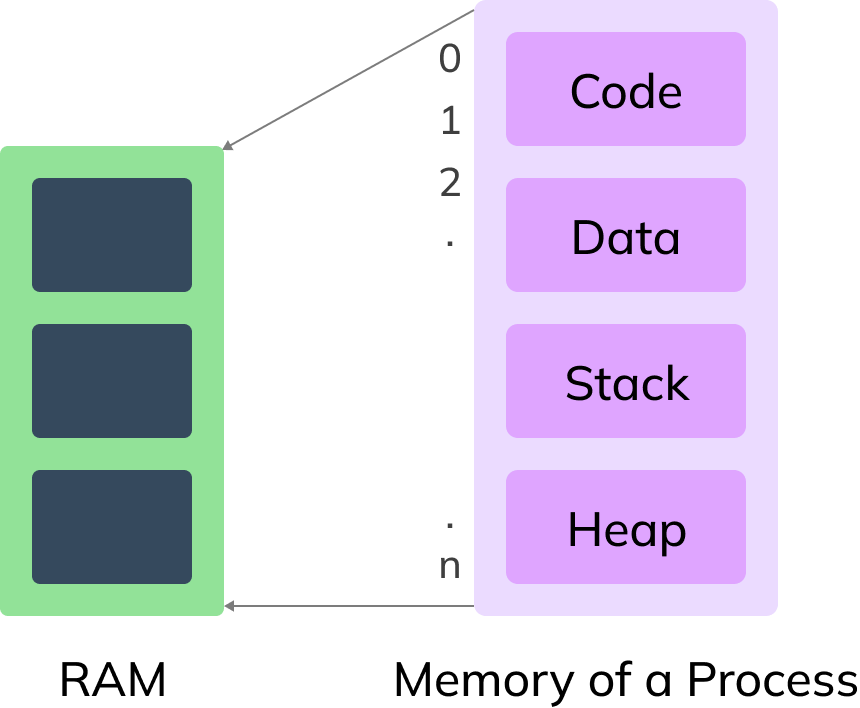
\includegraphics[width=0.6\columnwidth]{figures/Memory.png}
\end{figure}
\begin{itemize}[topsep=-0.5em, parsep=0.5em]
   \item	OS \rgbR{manages process memory}: code, data, stack, heap.
   \item	Each \rgbR{process perceives} a dedicated memory space starting from 0 (virtual addresses).
   \item	OS \rgbR{abstracts} actual memory placement and translates virtual addresses to physical addresses.
\end{itemize}


\columnbreak

\subsection*{States of a process}
\begin{figure}[H]
   \centering
   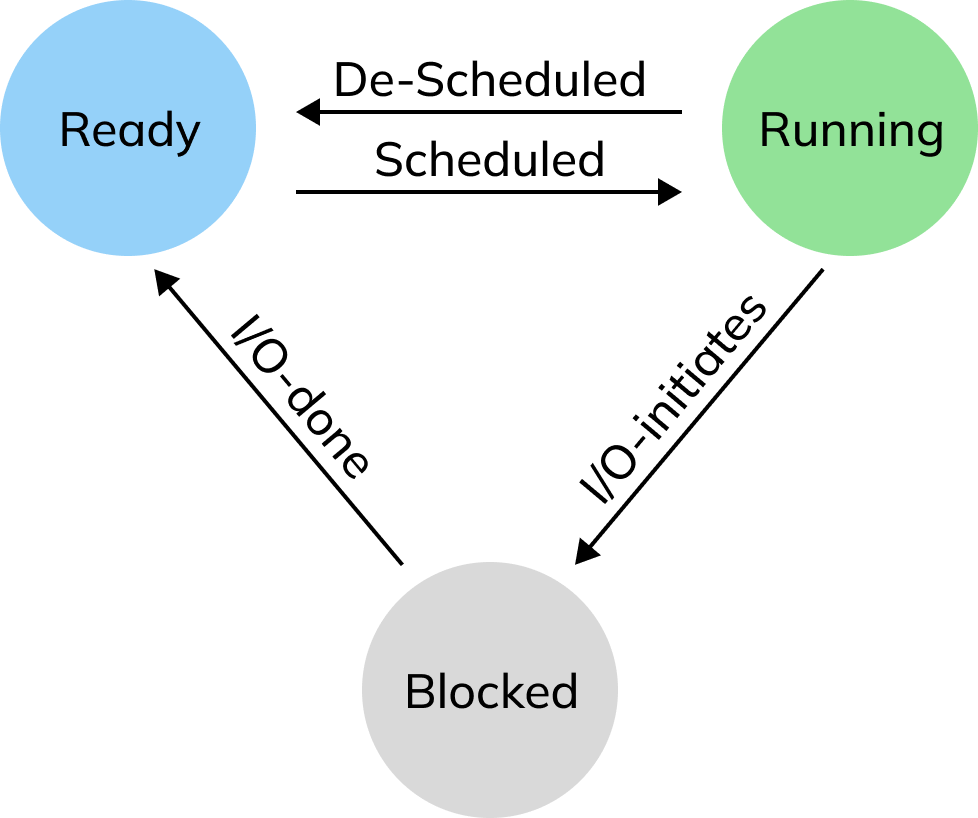
\includegraphics[width=0.6\columnwidth]{figures/States of Process.png}
\end{figure}

\vspace{-\baselineskip}
\begin{tabular}{ll}
   {Running} &: currently executing on CPU \\
   {Ready}   &: waiting to be scheduled \\
   {Blocked} &: suspended, not ready to run \\
   {New}     &: being created, yet to run \\
   {Dead}    &: terminated \\
\end{tabular}

Example:\\[0.5em]
\begin{tabularx}{\linewidth}{|c|c|c|C|}\hline
   Time & $P_0$ & $P_1$ & Note \\\hline
   1 & Running & Ready & \\\hline
   2 & Running & Ready & $P_0$ initiates I/O\\\hline
   3 & Blocked & Running &
   \makecell{$P_0$ is blocked\\$P_1$ is running}\\\hline
   4 & Ready & Running & $P_0$ I/O done\\\hline
   5 & Ready & Running & $P_1$ now done\\\hline
   6 & Running & - & $P_0$ now done\\\hline
\end{tabularx}


\subsection*{Process Scheduling}
\textbf{Queues:} processes migrate among the various queues -
\begin{itemize}[topsep=-0.5em, parsep=0.5em]
   \item \textbf{Job queue}: set of all processes in the system
   \item \textbf{Ready queue}: set of all processes residing in main memory, ready and waiting to execute
   \item \textbf{Device queues}: set of processes waiting for an I/O device
\end{itemize}

\vspace{1em}
\textbf{Types of Schedulers:}
\begin{figure}[H]
   \centering
   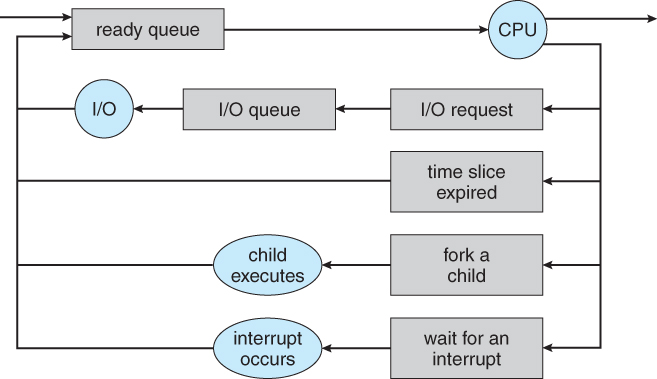
\includegraphics[width=\linewidth]{figures/Process Scheduling.png}
\end{figure}

\begin{itemize}[topsep=-0.5em, parsep=0.5em]
   \item	\textbf{Long-term scheduler (job scheduler):} selects which processes to brought into the ready queue; controls degree of multiprogramming.
   \item	\textbf{Short-term scheduler (CPU scheduler):} selects which process executes next and allocates the CPU.
\end{itemize}


\textbf{A Simple Function Call}

\begin{minipage}{0.6\linewidth}
\begin{itemize}[topsep=-0.5em, parsep=0.5em]
	\item	Function call \rgbR{translates} to a jump instruction.
	\item	\rgbR{New stack frame} is pushed and SP updated.
	\item	\rgbR{Old PC value} is pushed and PC updated.
	\item	Stack \rgbR{frame contains} return value, function arguments.
\end{itemize}
\end{minipage}%
\hfill
\begin{minipage}{0.28\linewidth}
   \centering
   \vspace{-1.5em}
   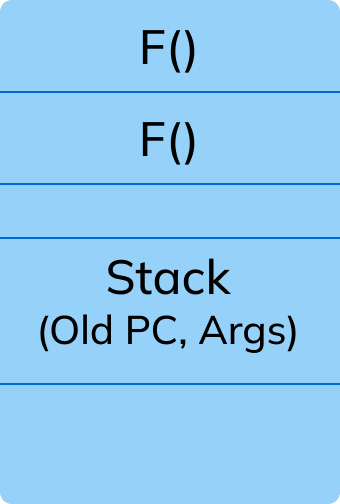
\includegraphics[width=0.8\linewidth]{figures/Function Call.png}
   \vspace{-1.5em}
\end{minipage}

\textbf{Why Switch Between Processes?}
\begin{itemize}[topsep=-0.5em, parsep=0.5em]
   \item OS in kernel mode may not return to the same process:
   \begin{itemize}
       \item Process has \rgbR{exited} or must be \rgbR{terminated}
       \item Process made a \rgbR{blocking system call}
   \end{itemize}
   \item OS may choose not to return to the same process:
   \begin{itemize}
       \item Process has \rgbR{run too long}
       \item CPU must be \rgbR{timeshared} with other processes
   \end{itemize}
\end{itemize}
In such cases, OS performs a \textbf{context switch} to switch between processes.

\subsection*{Mechanism of Context Switch}
Let's assume process $A$ moves from user to kernel mode; OS decides to switch from $A$ to $B$.

\begin{itemize}[topsep=-0.5em, parsep=0.5em, leftmargin=1em]
   \item \rgbR{Save} context of \rgbR{A} (PC, registers, kernel stack pointer) on A's kernel stack.
   \item \rgbR{Switch SP to B}'s kernel stack.
   \item \rgbR{Restore} context from \rgbR{B}'s kernel stack.
   \item \rgbR{Registers} on B's kernel stack were saved by OS when B was previously switched out.
   \item CPU now runs B in kernel mode; \textbf{return-from-trap} switches to B's user mode.
\end{itemize}

\columnbreak


\subsection*{Shared Memory}
\begin{itemize}[topsep=-0.5em, parsep=0.5em, leftmargin=1em]
   \item	Processes can \rgbR{access} the same memory region via \texttt{\rgbR{shmget()}} system call.
   \item	Using the \rgbR{same key}, two processes get the same memory segment.
   \item	Processes can \rgbR{read/write to communicate}.
   \item Process must ensure \rgbR{not to overwrite} the other's data (e.g., use synchronization).
\end{itemize}

\subsection*{Pipes}
\begin{figure}[H]
   \centering
   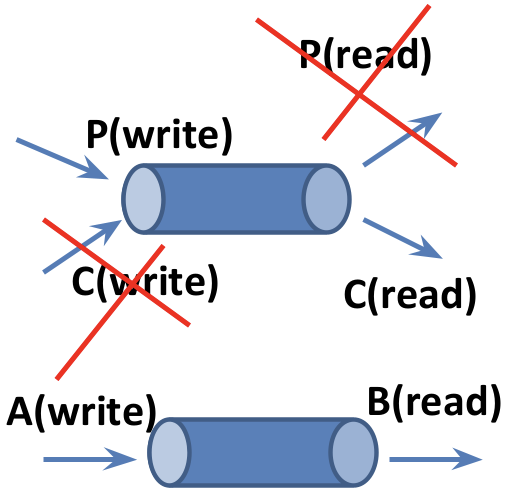
\includegraphics[width=0.4\linewidth]{figures/Pipes.png}
\end{figure}
\begin{itemize}[topsep=-0.5em, parsep=0.5em, leftmargin=1em]
    \item Returns two file descriptors: \textbf{read handle} and \textbf{write handle}.
    \item Pipes are \textbf{half-duplex communication}: data written to one fd can be read from the other.
    \item \textbf{Regular pipes}: both fds in the same process. Useful because parent and child share fds after \texttt{fork()}: parent uses one end, child uses the other.
    \item \textbf{Named pipes}: endpoints can be in different processes.
    \item Pipe data is buffered in OS between write and read.
\end{itemize}

\subsection*{Message Queues}
\begin{itemize}[topsep=-0.5em, parsep=0.5em, leftmargin=1em]
    \item Provide a \textbf{mailbox abstraction}.
    \item Processes can open a mailbox at a specified location.
    \item Processes can send/receive messages via the mailbox.
    \item OS buffers messages between send and receive.
\end{itemize}

\end{multicols}